\documentclass[conference]{IEEEtran}

\usepackage{cite}
\usepackage{url}
\usepackage{tipa}
\let\ipa\textipa
\ifCLASSINFOpdf
  \usepackage[pdftex]{graphicx}
  \DeclareGraphicsExtensions{.pdf,.jpeg,.png}
\else
  \usepackage[dvips]{graphicx}
  \DeclareGraphicsExtensions{.eps}
\fi
\graphicspath{{figures/}}
\usepackage[caption=false,font=footnotesize]{subfig}

%\usepackage[cmex10]{amsmath}
%\interdisplaylinepenalty=2500
%\usepackage{algorithmic}
%\usepackage{array}
%\usepackage{mdwmath}
%\usepackage{mdwtab}
%\usepackage{eqparbox}
%\usepackage{fixltx2e}
%\usepackage{stfloats}

% correct bad hyphenation here
% \hyphenation{op-tical net-works semi-conduc-tor}

\begin{document}
\title{Modeling Speech Production Using\\
  the Neural Engineering Framework}

\author{\IEEEauthorblockN{Bernd J. Kr\"{o}ger}
\IEEEauthorblockA{Neurophonetics Group,\\
Department for Phoniatrics, Pedaudiology,\\
and Communication Disorders,\\
Medical School, RWTH Aachen University, Germany\\
Email: bkroeger@ukaachen.de}
\and
\IEEEauthorblockN{Trevor Bekolay and Chris Eliasmith}
\IEEEauthorblockA{Centre for Theoretical Neuroscience,\\
University of Waterloo, Canada\\
Email: \{tbekolay, celiasmith\}@uwaterloo.ca}}

\maketitle

\begin{abstract}
  A neurobiologically plausible model of speech production is
  introduced here using the Neural Engineering Framework (NEF).
  This approach allows
  detailed modeling of temporal aspects of action selection and action
  execution in speech production  at the level of single spiking neurons.
  A preliminary architecture of our
  NEF speech production model is introduced and discussed in
  the second part of this paper. The first part focuses on an
  articulatory-acoustic model, generating acoustic speech signals on
  the basis of articulatory geometries. Our approach uses a small set
  of functional articulatory control parameters. Motor
  planning is based on the concept of speech or vocal tract actions
  (Kr\"{o}ger et al. 2010, Cognitive Processing 11: 187-205). A
  2D-geometrical model is used and the acoustic speech signal is
  calculated using a reflection-type line analog model.
\end{abstract}

\IEEEpeerreviewmaketitle

\section{Introduction}

Different approaches exist for describing the speech production
hierarchy. However, in general it is thought that
cortical processing starts with conceptualization of the
communicative act, followed by lexical retrieval of words, and its
syntactic processing. Subsequently, a phonological sound sequence is
encoded for the planned utterance (e.g. \cite{levelt1999}). At lower
levels of speech production, the phonological representation activates
syllable-level motor plans mainly in premotor cortical areas, which is
followed by motor execution, involving primary motor areas,
cerebellum, basal ganglia, and the motor neuron system of
speech articulators \cite{riecker2005}. Subsequently, a temporal
succession of vocal tract shapes and acoustic speech signals are
generated by the peripheral vocal tract system.

In this paper, we first describe an articulatory-acoustic model
that focuses on the lower levels of speech production.
Then, we describe an architecture for the higher levels
of speech production that can be realized
using the Neural Engineering Framework \cite{eliasmith2003},
and can be used to generate signals that
will drive the articulatory-acoustic model.

Input units for our articulatory-acoustic model
are speech or vocal tract actions
\cite{kroger1993,kroger2010}. These actions define a sequence of vocal
tract shapes. The most important information extracted from each vocal
tract shape, i.e. from each set of positions
for the speech articulators, is the
shapes of vocal tract cavities, which serve as the basis for the
generation of the acoustic speech signal \cite{kroger1993}.

\section{The Action-Based Approach for Controlling Speech
  Articulation}

Based on previous work \cite{saltzman1989,goldstein2006}, we assume
\textit{vocal tract action units} (also called speech actions or
speech gestures) as the basic motor planning units in speech
production \cite{kroger2010}. From the viewpoint of speech learning, it
is evident that infants babble a multitude of
\textit{gross vocal tract actions} in their first year,
mainly leading to successions of
vocal tract opening and closing actions,
which can sound, for example,
like \ipa{[bAbA]}, \ipa{[dAdA]} or \ipa{[gAgA]}
\cite{kroger2009,kroger2014}. Thus, we
can start by separating vocal tract \textit{opening actions} and vocal
tract \textit{closing actions}. Vocal tract opening actions can also
be called \textit{vocalic actions}, because opening actions result in
vowel-like sounds. Vocal tract closing actions are also called
\textit{consonantal actions}, because closing actions
lead to local vocal tract constrictions
as are part of consonant-like sounds,
e.g. produced by the lips, by the tongue dorsum, or by
the tongue tip. In addition, infants are capable of producing
\textit{velopharyngeal ab- and adduction actions} (lowering and
raising the velum), which separate nasal from
non-nasal sounds, and \textit{glottal ab- and adduction actions},
which separate voiced from voiceless sounds \cite{kuhl2004}.
Vocal sounds produced in these ways are not
necessarily language specific but result from an infant's exploration of
the vocal tract (i.e., babbling).

All types of vocal tract actions resulting from babbling are listed in
Table~\ref{tab:actions} and it is the main goal of speech learning
to 1) fine tune these (gross) vocal tract actions with respect to
\textit{spatial} as well as to \textit{temporal intra-vocal tract
  action parameters} in order to later on produce
different vowels and consonants of a specific target language, and to
2) fine tune the temporal coordination between different vocal tract
actions by varying \textit{inter-vocal tract action parameters} with
respect to the specific prosodic characteristics of that target
language. These parameters determine the temporal location of
consonantal, velopharyngeal and glottal actions with respect to
vocalic speech actions. An example for the temporal ordering of a
monosyllabic word, ``palm,'' produced by our control method is given in
Figure~\ref{fig:actions}. In our current model, the
\textit{intra-action temporal control} as well as the
\textit{inter-action timing} is defined by values for the beginning
and ending of onset-, target- and offset-time interval for each vocal
tract action. These time instants are elucidated in
Figure~\ref{fig:actions} for all speech actions forming the word
``palm''. During the \textit{onset time interval}, articulators move
towards the spatial action target, e.g. to lip closure in the case of a
labial closing action or to an open vocal tract shape in the case of the
vocalic action in ``palm''. This (partial) vocal tract target shape is
held during the \textit{target time interval}
(e.g. the lips are held closed during
the target time interval of the \ipa{[p]} in ``palm'')
and released at the beginning of the \textit{offset time interval}.

\begin{table}[!t]
\renewcommand{\arraystretch}{1.3}
\caption{Types of vocal tract actions, their spatial intra-vocal tract
  action parameters, and examples for potential speech sounds (symbols
  in parentheses []) or speech sound features which can be produced
  after learning a correct parameter specification.}
\label{tab:actions}
\centering
\begin{tabular}{l|p{2.5cm}|p{4cm}}
  type of action & spatial parameters & examples (after fine-tuning of
  actions)\\
  \hline
  vocalic & high-low & high: \ipa{[i, u, y]}; low: \ipa{[A]}\\
  ~ & back-front & back: \ipa{[u]}; front: \ipa{[i, y]}\\
  ~ & spread-rounded & spread \ipa{[i]}; rounded: \ipa{[u, y]}\\
  \hline
  consonantal & end-effector & lips: \ipa{[b, p, f, m]};
  tongue tip: \ipa{[d, t, s, n, l]}; tongue dorsum: \ipa{[k, g]}\\
  ~ & degree (type) of constriction &
  full closure: \ipa{[b, p, m, d, t, n, k, g]} (plosives and nasals) \newline
  near closure: \ipa{[f, s, S]} (fricatives) \newline
  lateral closure: \ipa{[l]}\\
  ~ & location of constriction & in case of tip: \ipa{[s]} in ``saw''
  vs. \ipa{[S]} in ``show''\\
  \hline
  velopharyngeal & abduction & nasal speech sounds: \ipa{[m, n]}\\
  ~ & adduction & non-nasal speech sounds (vowels, plosives, fricatives,
  ...)\\
  \hline
  glottal & abduction & voiceless speech sounds: \ipa{[p, t, k, f, s, S]}\\
  ~ & adduction & voiced speech sounds: \ipa{[b, d, g, m, n, l]} and all
  vowels\\
  pulmonic & pressure (resulting from movements of chest and diaphragm)
  & one action per utterance; constant pressure;
  degree of that pressure determines speech intensity of whole utterance
\end{tabular}
\end{table}

\begin{figure}[!t]
\centering
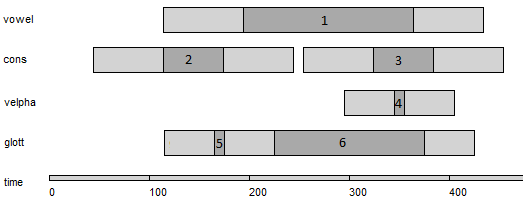
\includegraphics[width=\columnwidth]{actions}
\caption{Vocal tract action score of the word ``palm'' \ipa{[pAm]}. Vocal
  tract actions are ordered with respect to four tiers (vocalic,
  consonantal, velopharyngeal, and glottal). Temporal location of
  onset (light gray), target (dark gray), and offset time intervals
  (light gray) for all six vocal tract actions of the word are shown.
  1: vocalic action with low spatial target position; 2: labial full
  closing action; 3: labial full closing action; 4: velopharyngeal
  abduction action; 5: glottal abduction action; 6: glottal adduction
  action. The offset time interval for action 5 overlaps with the
  onset time interval of action 6. Time scale (bottom) is in milliseconds.
  Thus, actions 1 and 6 lead to \ipa{[A]}, actions 2 and 5 lead to
  \ipa{[p]}, and actions 3, 4, and 6 lead to \ipa{[m]}.
  The temporal overlap of vocal tract
  actions can also be called coarticulation.}
\label{fig:actions}
\end{figure}

\section{Control Parameters, Vocal Tract Shapes, and Area Functions}

Our set of articulatory control parameters is small but
\textit{functional} from the viewpoint of speech production. Three
vocalic parameters (\textit{front-back}, \textit{high-low}, and
\textit{spread-rounded}) control the overall shape of the vocal tract,
as is needed for the production of all vowels. For example, \textit{high-low} separates
vowels like \ipa{[i, y, u]} from \ipa{[A]} (vocal tract shapes for these vowels are given in
Figure~\ref{fig:sagi}, top row). The consonantal parameters (\textit{lip
  adduction}, \textit{tongue tip elevation}, \textit{tongue body
  elevation}) control \textit{degree (or type)} of consonantal
constrictions (e.g. full-closure in case of plosives or nasals, near
closure in case of fricatives, lateral closure in case of laterals).
Full-closure of the \textit{lip adduction} parameter
leads to production of \ipa{[p, b, m]}; full-closure of the
\textit{tongue tip elevation} parameter leads to production of
\ipa{[d, t, n]}; and full-closure of the \textit{tongue body elevation} parameter
leads to production of \ipa{[k, g]} (see also Table~\ref{tab:actions}).
Near-closure of the \textit{lip adduction} parameter leads to production
of \ipa{[f]}; near-closure of the \textit{tongue tip elevation} parameter leads
to production of \ipa{[s, z, S, Z]}; and near-closure of the
\textit{tongue body elevation} parameter leads to production of \ipa{[x]}.
Thus, while vocalic parameters control the overall shape of vocal tract,
consonantal parameters control local parts
of the vocal tract shape (e.g. the lip, tongue tip, or tongue
dorsum regions; see Figure~\ref{fig:sagi}, bottom row). In addition, the
parameters \textit{glottal abduction} and \textit{velopharyngeal abduction}
control the position of the vocal folds
and of the velum respectively.

As opposed to complex models,
in which the \textit{shape of the vocal tract} is
generated on the basis of modeling muscle activations and the tissue structures of
speech articulators (e.g. \cite{dang2004}), our approach is purely
geometrical. The contours of speech articulators are described by the
2D locations of 14 contour points for the upper lips, 17 points for
the lower lips, 23 points for the tongue,
15 points for the hard palate, 34 points for the velum,
and 23 points for the pharynx wall, larynx, and epiglottis.
These 2D locations are obtained from static MRI scans
for three contours representing the (extremal) cardinal vowels \ipa{[i]}, \ipa{[A]},
\ipa{[u]} (see \cite{kroger2005,kroger2004}). It is assumed that all vowel
shapes can be generated by interpolating between these extremal contours
using the three \textit{vocalic control parameters} introduced above.
In addition, extremal contours are generated for maximal labial
adduction, maximal elevation of the tongue tip, and
maximal elevation of the tongue dorsum.
Consonantal vocal tract shapes
within the local regions of constriction are
determined by interpolating between the current underlying vocalic
tract shape and the current consonantal extremal contours.
In addition to the \textit{degree of constriction} (see above),
one more parameter is needed for the
tongue tip, which controls the \textit{place of articulation},
in order to differentiate between alveolar and postalveolar tongue tip
constrictions (e.g. \ipa{[s]} or \ipa{[S]}; see Table~\ref{tab:actions}). The
exact location for tongue dorsum closure is controlled indirectly by
the current value of the vocalic front-back parameter.

\begin{figure*}[!t]
\subfloat[\ipa{[A]}]{
  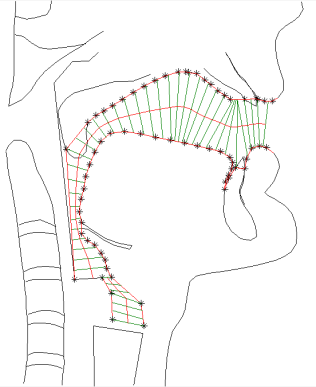
\includegraphics[width=0.2\textwidth]{sagi1}
  \label{fig:sagi1}
}
\hfil
\subfloat[\ipa{[i]}]{
  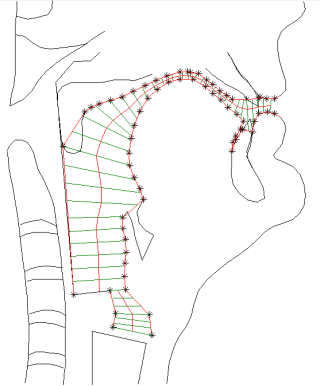
\includegraphics[width=0.2\textwidth]{sagi2}
  \label{fig:sagi2}
}
\hfil
\subfloat[\ipa{[u]}]{
  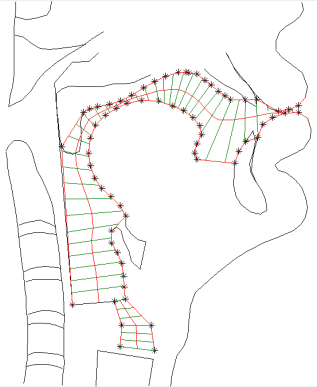
\includegraphics[width=0.2\textwidth]{sagi3}
  \label{fig:sagi3}
}
\hfil
\subfloat[neutral]{
  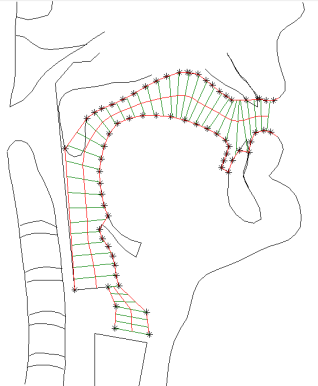
\includegraphics[width=0.2\textwidth]{sagi4}
  \label{fig:sagi4}
} \vspace{-1em}

\subfloat[area function for \ipa{[A]}]{
  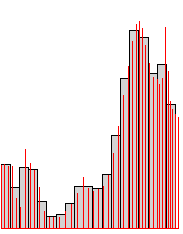
\includegraphics[width=0.2\textwidth]{sagi5}
  \label{fig:sagi5}
}
\hfil
\subfloat[lips closure]{
  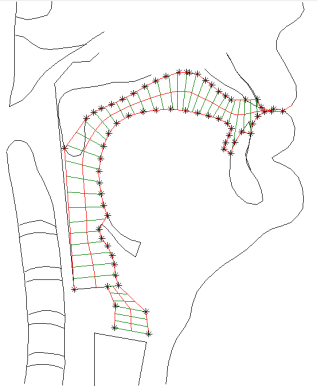
\includegraphics[width=0.2\textwidth]{sagi6}
  \label{fig:sagi6}
}
\hfil
\subfloat[tongue tip closure]{
  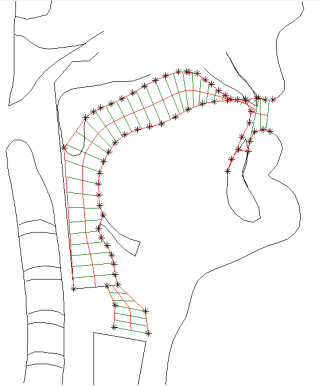
\includegraphics[width=0.2\textwidth]{sagi7}
  \label{fig:sagi7}
}
\hfil
\subfloat[tongue dorsum closure]{
  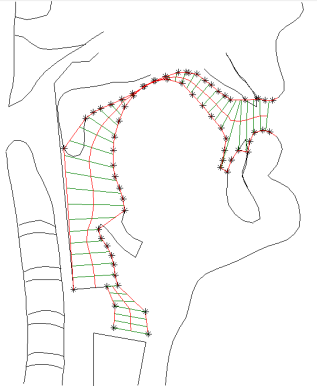
\includegraphics[width=0.2\textwidth]{sagi8}
  \label{fig:sagi8}
}
\caption{Top row: vocalic midsagittal views. These vocalic views
  reflect a change in the shape of the entire vocal tract.
  Bottom row: midsagittal views of consonantal closures.
  These views reflect a change in the shape of a local area
  of the vocal tract, and can therefore be combined
  with the global shape defined by the vocalic context.}
\label{fig:sagi}
\end{figure*}

While no coarticulatory corrections are needed for the interpolation
of vocalic contours (i.e., lip rounding can be independently controlled
from tongue positioning without causing any problems in our
geometrical model), two coarticulatory corrections are needed in the
case of consonantal articulation. (1) In the case of producing a
labial constriction (increasing lip adduction), the front part of
tongue needs to be elevated, because lip adduction implies an
elevation of lower jaw. (2) In the case of producing an apical
constriction (raising the tongue tip), spatial coarticulation
needs to be high for high vowels. Here, the contour of
consonantal closure needs to be influenced strongly by the current
underlying vocalic vocal tract shape. In our model, this problem is
solved by introducing different consonantal target shapes based on the
current vocalic coarticulation (see also \cite{kroger2004}).

For calculating the \textit{vocal tract area function}, i.e. vocal tract
cavity information from a vocal
tract shape, a lower line, upper line, and midline are defined
(red lines in the midsagittal views of Figure~\ref{fig:sagi}).
The lower line represents the front-low margin,
and the upper line the back-high margin of
the vocal tract cavity (vocal tract tube) from larynx to lips.
The midline defines the midline for air to flow through
the vocal tract tube from glottis to lips.
While the lower and upper lines are defined by vocal
tract contour points (black asterisks in Figure~\ref{fig:sagi}),
the calculations of the midline and the green distance lines
(see Figure~\ref{fig:sagi}) are done in a complex iterative procedure.
A set of \textit{42 distance lines} is defined;
these lines are perpendicular to the midline and thus perpendicular to the
airstream within the vocal tract tube (green lines in
Figure~\ref{fig:sagi}). These distance lines are the basis for
calculating the area function (an example of an area function is
given in Figure~\ref{fig:sagi5}) for the vocal tract shape of \ipa{[A]}. (cf.
\cite{perrier1992}).

\section{Modeling Vocal Tract Acoustics}

Input for the calculation of the acoustic speech signal is the area
function and glottal flow. The glottal flow is calculated using an
LF-model derivate \cite{veldhuis1998}. Flow and pressure values within
the vocal tract are calculated using a reflection-type line analog
\cite{liljencrants1985}. Here, the geometry of the vocal tract tube is
``digitized'' into a succession equidistant cylindrical tubes (see
the gray bars, representing the area function, in
Figure~\ref{fig:sagi5}). The length of each tube segment is 0.875 cm
in our case of 20 kHz sampling frequency for the acoustic signal. Flow
and pressure values are calculated for each tube segment at each time
instant. Acoustic and aerodynamic loss mechanisms including losses due
to sound radiation at the mouth are included \cite{liljencrants1985}.
Because the length of the vocal tract and thus the number of tube
segments varies with respect to overall tube length (e.g. longer tract
length and thus more tube segments for \ipa{[u]} compared to \ipa{[i]}
or \ipa{[A]}), and because the reflection-type line analog cannot handle
varying tube length easily, the vocal tract shape over time is
evaluated only once per glottal pulse (glottal period) and is
thus assumed to be constant for that time period. The
resulting radiated sound signal (pulse response) is calculated over a
time interval of two glottal periods (see Figure~\ref{fig:signal}) and is
overlayed pulse by pulse in time, in order to form the resulting speech
sound signal.

\begin{figure}[!t]
  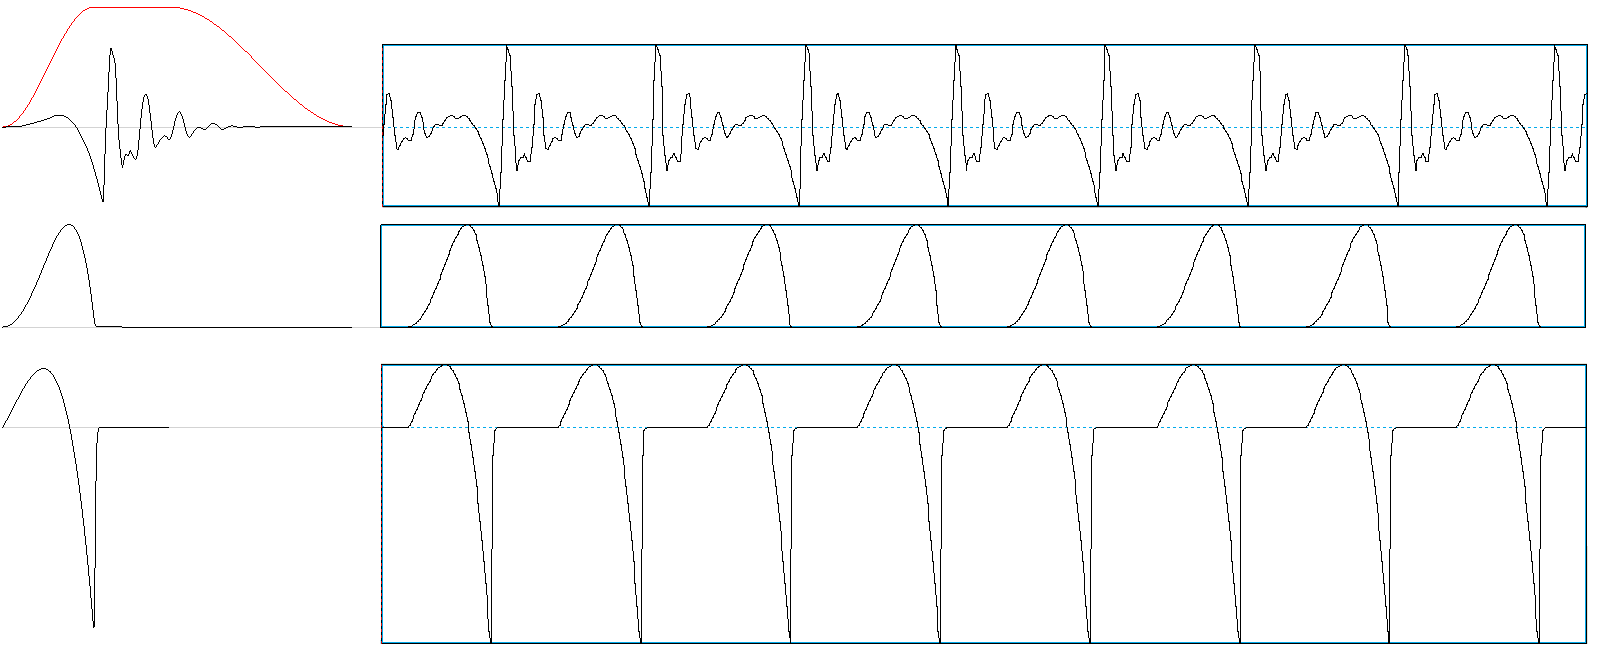
\includegraphics[width=\columnwidth]{signal1234}
  \caption{Left side: single glottal pulse (middle: glottal flow;
    bottom: its time derivative for exactly one glottal period) and
    pulse answer for an \ipa{[A]}, radiated from mouth (top). Right side
    top: acoustic speech signal, resulting from overlayed pulse
    answers; middle: glottal flow waveshape for 9 glottal cycles;
    bottom: first time derivative of glottal flow. The Hanning window
    for temporal overlay of pulse responses is asymmetric. Onset ends
    at the time instant of maximum glottal excitation (i.e. negative peak
    of time derivative of glottal flow) and offset interval begins at
    end of glottal cycle. Right side signals are displayed using
    the PRAAT software to visualize the WAV file generated by our
    synthesizer; left side signals are displayed from the synthesizer
    software directly.}
\label{fig:signal}
\end{figure}

\section{The Neural Engineering Framework}

The Neural Engineering Framework (NEF; \cite{eliasmith2003})
provides three principles for \textit{representing} and
\textit{transforming} information \textit{dynamically}
using feedforward and recurrently connected networks
of spiking neurons.
Nengo is a neural simulation environment that uses the NEF
to build large-scale brain models \cite{bekolay2014}.
The NEF and Nengo have been used to create models of visual
object recognition and copy drawing of manually drawn digits by
performing visual perception, cognitive tasks, and motor tasks
with networks of spiking neurons \cite{eliasmith2012,eliasmith2013}.
These cognitive and sensorimotor tasks are performed by
complex brain models which are made up of many networks representing
cortical circuits, basal ganglia, thalamus, as well as peripheral
sensory processing and motor outputs.
Each of these models uses a simulated spiking neuron approximation,
usually LIF (leaky-integrate-and-fire) neurons
(see \cite{eliasmith2013}, p. 35ff).
Moreover, many of the models created with the NEF
use a cortex-basal ganglia-thalamus-cortex loop
that is capable of modeling action
selection and action execution, as is needed in order to simulate
communication (e.g. question-answering scenarios).

We believe that this approach can be used to model speech
production, because its action selection and
execution mechanisms can be extended or modified
and thus can meet the demands occurring in face-to-face interactions;
see \cite{kroger2011}. In the next section of this paper,
a preliminary architecture for speech production is introduced.

\section{The architecture of the speech production model}

A speech production model should be made up of a cognitive component
(mental lexicon) as well as a sensorimotor component (speech action
repository, SAR, and a production-perception loop; see
\cite{kroger2009,kroger2014,kroger2012,kroger2011a,eckers2013,eckers2013a,kroger2010}).
It is a key feature of our ongoing work on modeling speech production
that phonological representations arise during
early phases of speech acquisition and are not predefined in the model
at the beginning
\cite{kroger2009,kroger2014,kroger2011}. Lexical items (semantic as
well as phonological representations) and phonetic (i.e.
hypermodal sensorimotor) representations of syllables within the
speech action repository
\cite{kroger2012,kroger2011a,eckers2013,eckers2013a,kroger2010} can be
represented in the NEF using the semantic pointer architecture (SPA; see
\cite{eliasmith2013}, p. 77ff). The word ``semantic'' is not used in
the SPA in a narrow linguistics sense; semantic pointers do not
exclusively represent meanings of words, phrases or sentences
but can represent motor states (e.g. the motor plan
of a complete syllable or the motor plan of a
target-directed hand-arm gesture) or sensory states
(e.g. auditory states of syllables, words or phrases, visual states).
Thus, a semantic pointer in the SPA can be used to describe
discrete cognitive processing units as well as sensory and/or motor
states (e.g. phonetic states of syllables as are defined in the SAR
\cite{kroger2012,kroger2011a,eckers2013,eckers2013a,kroger2010}).

An advantage of the SPA is that it connects cognitive,
sensory, and motor states. A comprehensive brain model including
cognitive, sensory and motor modules called Spaun has been
developed with the NEF and Nengo (see \cite{eliasmith2012} and \cite{eliasmith2013}, p. 247ff).
Spaun uses visual information (an image of a hand-written digit)
to do eight tasks, including copy drawing,
pattern completion, and a reinforcement learning task
similar to gambling.
It provides its output by producing motor commands that
drive a simulated three-link arm to write digits.
We believe that the motor system of Spaun
can be augmented by a speech motor component, i.e. by a speech
articulator system, which can be implemented in parallel to the
already existing arm motor component. A discussion of similarities
and differences of controlling hand-arm motor system, articulator
motor system and facial motor system (in face-to-face communication
scenarios) is given in \cite{kroger2010}. Moreover, the perceptual
system within Spaun can be augmented by an auditory perceptual system
in order to allow speech acquisition and speech perception. This
auditory perceptual component can be implemented in parallel to the
already existing visual perceptual component (see
Figure~\ref{fig:model}).
Upon augmenting Spaun's sensory and motor modules,
similar cognitive tasks as are currently performed by Spaun
through seeing and writing digits
can instead be done by hearing and speaking
the words corresponding to those digits.

\begin{figure}[!t]
\centering
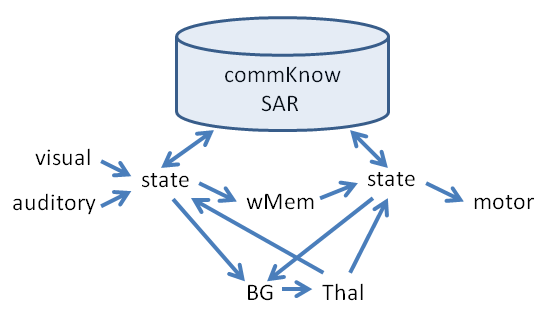
\includegraphics[width=\columnwidth]{model}
\caption{High-level NEF model architecture for syllable and word processing.
  ``commKnow'' and ``SAR'' represent a neural long-term knowledge
  (communicative knowledge like a mental lexicon, and syllable action
  repository). ``wMem'' represents the working memory, ``BG'' the
  basal ganglia network, and ``Thal'' the thalamus
  network. Semantic pointers can be activated and processed in both
  state networks on the basis of audiovisual input (left state
  network: perceptual state network) or at the level of motor planning
  (right state network: action planning network; see also text).}
\label{fig:model}
\end{figure}

One further advantage of Spaun is the neurobiological representation
of the cortex-basal ganglia-thalamus-cortex loop in order to model
action selection and control of perception-action tasks
(see \cite{eliasmith2013}, p. 163ff). We believe that the concepts
introduced by \cite{eliasmith2013} for control of
visual-perception-manual-action tasks are applicable in a similar way
for auditory-perception-articulatory-speech-action tasks.

Sensorimotor knowledge concerning the motor and auditory state of
syllables as well as a reference pointer towards the
phonemic representation of each syllable
is stored in the ``SAR'' (speech action repository) in form of
predefined (i.e. learned) semantic pointers (Figure~\ref{fig:model}).
Basic behavioral knowledge for face-to-face communication in speech
production scenarios is stored in the  ``commKnow'' (communicative knowledge)
module in form of predefined (i.e. learned) semantic pointers.
The mental lexicon as well is part of ``commKnow''.
Syllable state pointers (e.g., for representing the syllables
``ba'', ``da'', ``ga'') as well as semantic pointers of
communication scenarios (e.g., for representing actions like
``listen to a communication partner'', ``produce a syllable, word or
phrase'') can be activated at the level of the state networks
(Figure~\ref{fig:model})
based on neural representations stored in long term memory
and based on actual audiovisual input (for example from a
communication partner / interlocutor).
This information is processed
in working memory as well as in the
cortex-basal ganglia-thalamus-cortex loop in order to generate and
activate motor plans (right state network) and in order to directly
control motor execution for articulation.

The size of the network components depends on the tasks which need to
be performed. In order to perform a speech production task
(e.g. syllable sequencing) as well as a more complex task including listening to
a communication partner (e.g. a question answering task), the size of
each cortical state network is 3000 LIF neurons,
and the sizes of the visual, auditory, and motor components are
300 LIF neurons each. The size of the recurrent network representing
working memory is 1000 LIF neurons. The basal ganglia is comprised of
5 subnetworks with 600 LIF neurons each (3000 neurons in
total; see \cite{eliasmith2013}, p. 164ff). The thalamus is
composed of a network of 750 LIF neurons (see
\cite{eliasmith2013}, p. 169ff).

The structure of a syllable sequencing subnetwork
as is visualized by the Nengo GUI\footnote{
  The Nengo GUI visualizes networks created in Nengo
  \cite{bekolay2014}. It is currently under development
  at \url{https://github.com/ctn-waterloo/nengo_gui}}
is shown in Figure~\ref{fig:ipynb551_structure}.
Here, the input stimuli are predefined sequences of semantic pointers
which can be interpreted as visual input. This input sequence
directly activates the phonemic representation of the syllable.
This cortical state information forms the input signal for the
basal ganglia-thalamus part of the network. This part of the
network subsequently activates the premotor and auditory state
of the syllable sequence. It can be seen that due to the basal
ganglia-thalamus loop, the activation of the premotor and auditory
states are delayed by around 50 ms with respect to phonemic input
(see Figure~\ref{fig:ipynb551_output}).

\begin{figure}
\centering
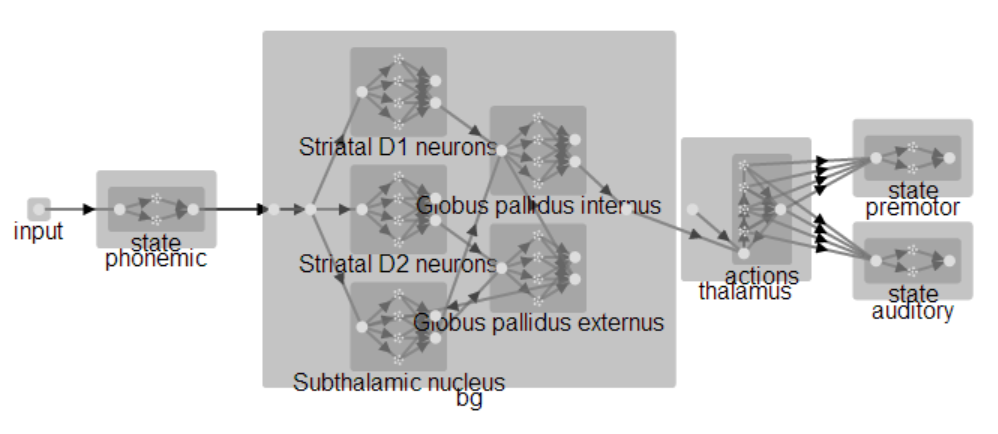
\includegraphics[width=\columnwidth]{ipynb551_structure}
\caption{Structure of the syllable sequencing network. ``bg''
  refers to the basal ganglia. The input semantic pointer is
  represented by the phonemic state network.
  That semantic pointer is communicated to premotor and auditory
  networks through a basal ganglia-thalamus network. See text
  for more details.}
\label{fig:ipynb551_structure}
\end{figure}

\begin{figure}
\centering
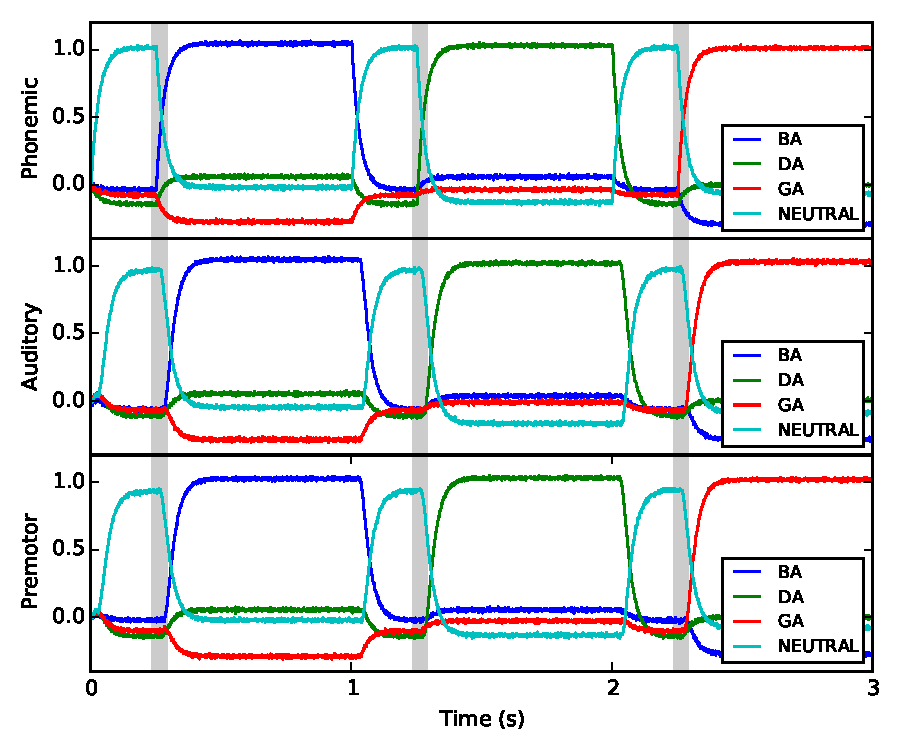
\includegraphics[width=\columnwidth]{ipynb551_output}
\caption{Information flow through the syllable sequencing
  network shown in Figure~\ref{fig:ipynb551_structure}.
  Information in the phonemic (top), auditory (middle),
  and premotor (bottom) populations are shown.
  Colored lines represent the similarity between the
  representation in the population and the target semantic pointer;
  the target semantic pointer is ``BA'' for the blue line,
  ``DA'' for the green line, ``GA'' for the red line,
  and ``NEUTRAL'' (i.e., no speech) for the cyan line.
  The shaded grey regions are 50 ms wide and show the delay
  between the phonemic and auditory/premotor representations.}
\label{fig:ipynb551_output}
\end{figure}

\section{Discussion and Further Work}

First steps in the direction of using the NEF, SPA, and Nengo
in order to model speech production and thus to contribute
to cognitive information communication issues
\cite{Baranyi2012} are
described in this paper. These tools are advantageous
for modeling speech production because this
approach operates in continuous time, and is robust to the
noise introduced by manipulating information with spiking neurons.
This allows us to model aspects of speech production
which are beyond the scope of other approaches. In particular,
aspects of face-to-face communication in speech due to
perception-action routing in the brain and specific aspects of speech
disorders due to different degrees of neural noise
can now be investigated in more detail.

We have also presented a functional articulatory-acoustic model.
This model is capable of modeling the processes of varying
intra- and inter-speech action parameters, i.e. for fine-tuning of
action targets, for action onset-, target-, and offset-interval
lengths, and for establishing the temporal relation between
different speech actions involved in
forming a syllable or word (cf. babbling and
imitation training \cite{kroger2009,kroger2014}). Because these
simulations demand the generation of an abundance of speech items,
our model is designed for generating speech items near real time.
Integrating nasal tract and noise sources for the generation of nasals
and fricatives respectively are the next tasks to be completed.
Then, we will conduct a study on the perceptual evaluation
of speech items produced by our model.

\IEEEtriggeratref{16}

\bibliographystyle{IEEEtran}
\bibliography{kroger}

\end{document}
